\chapter{Trusted Platform Module}
The Trusted Platform Module is a system component used as a cryptographic co-processor. The TPM specification was defined and is currently maintained by Trusted Computing Group (TCG), formerly known as Trusted Computing Platform Alliance. The specification was also standardized by International Organization for Specification (ISO) and International Electrotechnical Commission (IEC) as ISO/IEC 11889.

This chapter introduces the basic concepts pertaining to TPMs, summarizes the history of their development, describes the TPM 2.0 specification, and reports on research also with regard to their various use cases. 

\section{Basic concepts}
This section provides an overview of basic concepts mentioned throughout this work.

\subsection{Trust, trusted, and trustworthy}
The term "trust" has no uniformly formalized definition. Its interpretations vary even in the same field of studies such as computer science and its subfields. The most relevant one for our needs is the TCGs' definition which states that trust is "the expectation that a device will behave in a particular manner for a specific purpose" \cite{tcg_arch_overview}. It is, however, important to note that this definition does not mention anything about the device being worthy of our trust. We only expect the specific behavior and the device does not guarantee anything about its behavior. This means that a trusted device may fail us, whereas a trustworthy device is worthy of our trust and does not fail.

\todo{Describe goals & use-case for Trusted Computing}

\subsection{Attestation}

\subsection{Platform Configuration Registers}
Platform Configuration Registers (PCRs) are dynamic memory locations inside a TPM used to store integrity metrics of software and its configuration. These locations can only be updated using \texttt{extend} operation and also read for reporting or attestation. The \texttt{extend} operation makes use of the cryptographic hash function to combine the digest stored in the PCR and the new data. Cryptographic hash function map data of arbitrary size to the output of a fixed size. Such outputs are conventionally called hashes, message digests, or digests. These functions have one-way property: when given a message digest, it is difficult  to compute the message itself. The extend operation works in the following way:
\begin{align*}
    d_{n+1} = h(d_{n}\ ||\ data)
\end{align*}
\begin{itemize}
    \item $||$ is a concatenation of data in binary form
    \item $ d_{n} $ is a digest stored in PCR before \texttt{extend} operation
    \item $ d_{n+1} $ is a digest stored in PCR after \texttt{extend} operation
    \item $ data $ is binary data to extend by
    \item $ h $ is a cryptographic hash function
\end{itemize}

We can always recompute the final value if we possess the knowledge of members previously used in the chain and detect potential alterations.

\section{History}
In this section, a TPM specification's history of development will be described. Firstly, versions 1.1b and 1.2 will be shortly described. Then reasoning behind the latest version of the TPM specification, the TPM 2.0 specification, will be discussed. The TPM 2.0 specification itself is described in a separate \myref{Section}{sec:tpm2}.

\subsection{TPM 1.1b}
The first broadly used specification was TPM 1.1b, released in 2003. TPMs released under this specification already provided some essential functions found in modern TPMs, consisting of key generation of RSA key pairs, storage, secure authorization, and device-health attestation. Anonymous identity keys based on certificates were used in order to assure privacy. However, the certificates needed to be provided with the TPM, and any generation of such keys was available only upon owner authorization. To prove the origin of the keys generated by TPM anonymously, a privacy certification authority was created. PCRs provide the integrity of measurements collected during the system's boot sequence. Both PCRs and identity keys might be used to prove the health of the system's boot sequence~\cite[p.~2]{arthur2015practical}.

The hardware specification was not standardized in TPM 1.1b. This caused various incompatibilities. The TPMs across different vendors provided differing interfaces, which required different drivers. Pin-outs on the chips were not prescribed by any standard. Additionally, there were no countermeasures against dictionary attacks~\cite[p.~2]{arthur2015practical}.

\subsection{TPM 1.2}
While being in development from 2005 to 2009, the TPM 1.2 specification went through numerous releases. Regarding the need to store shipped certificates for TPM's endorsement keys on a hard disk, about 2KB of non-volatile RAM was added. A new design was needed to support key migration between different TPMs because the old design of key migration would in TPM 1.1b require users to have TPM owner authorization. The new idea enabled users to create migratable keys and then relied on a designated third party that could exclusively migrate such keys. Said keys could also be certified. Thus, they were called Certified Migratable keys. An internal timer able to synchronize with the external one was added in 1.2, which has its use when signing data due to timestamps. Version 1.2 required API to provide backward compatibility for 1.1b. This increased the complexity of the new specification. The TPM 1.2 became widely used in x86 personal computers starting in 2005 and later in 2008 also in servers~\cite[p.~3]{arthur2015practical}.

\subsection{TPM 2.0 reasoning}
One factor contributing to the need for yet another specification after TPM 1.2 was that in 2005, some substantial collision attacks were found against the SHA-1 hash function. Analysis regarding the use of SHA-1 in TPM revealed the attacks not being applicable~\cite{tcg_tpm1.12_sha-1_uses}. The SHA-1 hashing algorithm was used extensively in TPM 1.2. However, when its flaw was discovered, there was no way to replace it quickly. This problem fueled the idea that the new specification had to permit any hashing algorithm without making any changes to the specification. So-called digest agility. 

Another problem was the lack of a symmetric algorithm required in the TPM specification. The use of RSA for encryption of serialized data was impractical because RSA operations are slow. That's why it was decided that the following specification would adopt support for symmetric encryption, which is faster and more suitable for encryption of large byte streams. Having this many problems, an overhaul of the specification would be convenient~\cite[p.~4]{arthur2015practical}.



\section{TPM 2.0}\label{sec:tpm2}
The chance to overhaul the specification given to TPM 2.0 architects and developers, was turned into much more than support for digest agility and for symmetric cryptography algorithms. Support for algorithm agility was added which allows for various cryptographic primitives to be implemented with different algorithms. Authorization methods were unified and expanded, allowing for the building of complex authorization policies. TPM management was simplified in order for the TPM to be more useful to applications.

%First sentence is prob a nonsense
The main goal of the new specification was to provide a library describing features and commands available for implementation. This architecture allows designers to choose the required level of security, which may vary for different use cases. 

This section describes various types of TPMs, their basic features, and use cases.

\subsection{Types}
There is no single correct way how should TPM 2.0 be implemented. TPM specification does not dictate if a TPM should be implemented in hardware or software. Different usage scenarios may require a different type of TPM. The TPM specification only defines functionality to be adhered to by its implementations. 

According to \cite{tcg_tpm2_briefintro}, five types of a TPM are considered:

\begin{itemize}
    \item \textbf{Discrete TPM} is a hardware implementation of TPM specification. It is implemented as a standalone chip designed to be highly secure and tamper-proof. It can be used to protect even against very advanced attacks in security-critical infrastructures.
    \item \textbf{Integrated TPM} is still implemented in hardware, although as a part of a more complex chip, such as a CPU, which may have other responsibilities than security. They are not required to be tamper-resistant because such a requirement may immensely increase such chips' cost.
    \item \textbf{Firmware TPM} runs in the CPU's trusted execution environment (TEE), which protects and isolates the code and data along with providing confidentiality and integrity guarantees. Firmware TPM's security is very dependent on the TEE's security.
    \item \textbf{Virtual TPM} does not require a physical chip to be present. It entirely relies on the fact, that its users will be hypervisors, and the Virtual TPM itself will be isolated from the software running on the virtual machine to protect its code. 
    \item \textbf{Software TPM} is implemented as an emulator ideally used for testing and system prototyping purposes. It does not run inside of an isolated environment and may be prone to tampering.
\end{itemize}

\subsection{Features}
\subsubsection{Enhanced Authorization}

\subsection{Architecture}
Although there is no prescribed form of TPM in terms of hardware or software, the specification requires its implementations to possess several functional components for its operation~\cite{tcg_p1_architecture}. Selection of important building blocks of TPM is shown in \myref{Figure}{fig:tpm-arch-scheme}.

\begin{figure}[H]
    \centering
    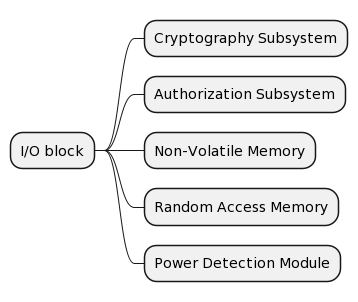
\includegraphics[width=\textwidth-6cm]{img/tpm-arch-diagram.png}
    \caption{Important blocks of TPM architecture}
    \label{fig:tpm-arch-scheme}
\end{figure}

\begin{itemize}

\item \textbf{I/O Buffer} is a location used for communication between the host platform and TPM. A precise description of interfaces used for communication is left up to designers of such interfaces.

\item \textbf{Cryptography Subsystem} which provides implementations of various cryptographic primitives, most of which may be used by other modules. These primitives generally consist of: 
\begin{itemize}
    \item Hash functions which may be used by external software, different TPM operations such as PCR extend, or other cryptographic primitives. 
    \item Symmetric cryptography provides means of symmetric encryption and decryption along with various block cipher modes of operation.
    \item Asymmetric cryptography is used for signatures, signature verification, and shared secret establishment. The only supported algorithms are RSA and ECC.
    \item Message Authentication Codes use either the beforementioned hashing capabilities (HMAC) or symmetric ones (SMAC).
    \item Random Number Generator is used as a source of randomness in TPM. The randomness is necessary for the generation of nonces and keys and for signatures. 
    \item Key Generation uses RNG value either directly as a secret key or as a seed to derive from applying some approved key derivation function.
\end{itemize}

\item \textbf{Authorization Subsystem} which tests that each executed command has required authorization to access Shielded Locations. 

\todo{Explain Shielded Locations}
\item \textbf{Non-Volatile Memory} provides persistent storage space for allocation and contains Shielded Locations.

\item \textbf{Random Access Memory} provides storage space that is not required to be persistent. It also contains Shielded Locations, most notably PCRs of which accumulative property is used to process logs of system state which may be subsequently validated. This is particularly useful when we want to measure the boot sequence of the system so that no malicious changes may be applied to it.

\item \textbf{Power Detection Module} handles TPM power states according to platform power state changes.
\end{itemize}

\section{Use cases}

\section{Research}

%\subsection{tpm2-algtest}
%The \texttt{tpm2-algtest}\footnote{https://github.com/crocs-muni/tpm2-algtest} is a tool for automatic gathering of information about the TPM2 devices \cite{Struk2019thesis}. The tool uses libraries implementing Trusted Computing Group's TPM2 Software Stack\footnote{https://github.com/tpm2-software/tpm2-tss} which allows for simplification of development when programming applications supposed to interact with the TPM. The tool tests for support of specific commands and supporting routines, values of structures defined in the TPM 2.0 specification \cite{tcg_p3_commands, tcg_p4_supproutines, tcg_p2_structures}. Supported cryptographic algorithms are also subject to performance analysis where the time to execute such an algorithm is repeatedly measured and recorded. Additionally, the tool uses the TPM to generate key pairs for RSA and ECC-based algorithms so that they can be further analyzed by various means.
